\documentclass[11pt,landscape]{article}
\usepackage{geometry} % Pour passer au format A4
\geometry{hmargin=1cm, vmargin=0.6cm} % 

% Page et encodage
\usepackage[T1]{fontenc} % Use 8-bit encoding that has 256 glyphs
\usepackage[english,french]{babel} % Français et anglais
\usepackage[utf8]{inputenc} 

\usepackage{lmodern}
\setlength\parindent{0pt}

% Graphiques
\usepackage{graphicx,float,grffile}

% Maths et divers
\usepackage{amsmath,amsfonts,amssymb,amsthm,verbatim}
\usepackage{multicol,enumitem,url,eurosym,gensymb}

% Sections
\usepackage{sectsty} % Allows customizing section commands
\allsectionsfont{\centering \normalfont\scshape}

% Tête et pied de page

\usepackage{fancyhdr} 
\pagestyle{fancyplain} 

\fancyhead{} % No page header
\fancyfoot{}

\renewcommand{\headrulewidth}{0pt} % Remove header underlines
\renewcommand{\footrulewidth}{0pt} % Remove footer underlines

\newcommand{\horrule}[1]{\rule{\linewidth}{#1}} % Create horizontal rule command with 1 argument of height

%----------------------------------------------------------------------------------------
%   Début du document
%----------------------------------------------------------------------------------------

\begin{document}



\setlength{\columnseprule}{1pt}

\horrule{2px}
\section*{DM - Modélisation du monde}
\horrule{2px}
\vspace{-1cm}

\subsection*{Les grands scientifiques - Congrès de 1927 - Solvay}

Après avoir entouré votre scientifique (Fait en classe !). 

\textbf{Marquer son nom, son prénom en gros, mettre une photo, la date et le lieu de naissance et marquer quelques phrases sur leurs domaines d'études ou découvertes.}

    \begin{figure}[H]
        \centering
        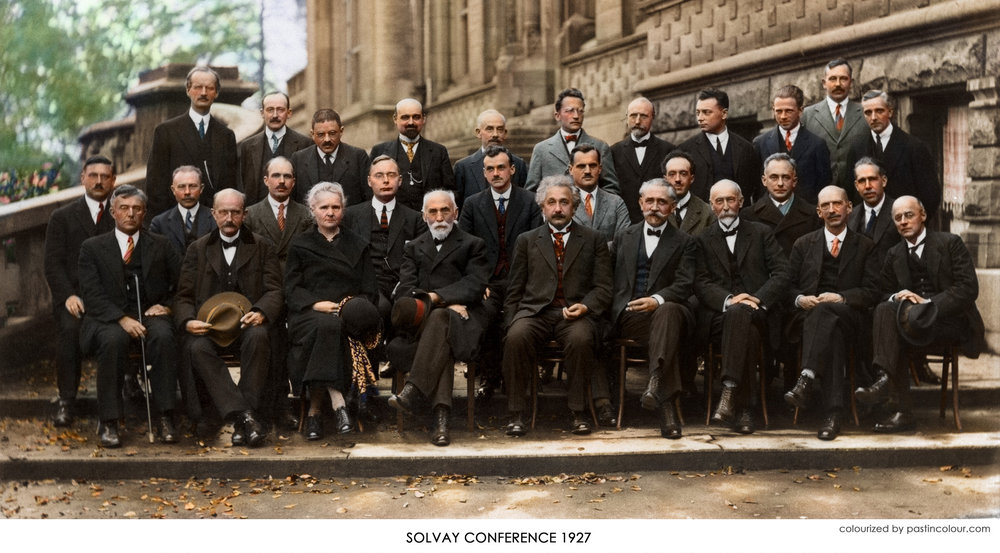
\includegraphics[width=0.8\linewidth]{4x5-calcul-litteral-1/sources/solvay.png}
  \end{figure}

\begin{center}
\textsc{A. Picard, E. Henriot P. Ehrenfest, Ed Hersen, Th de Donder, E. Schrödinger, E. Verschaffelt, W. Pauli, W. Heisenberg, R.H. Fowler, L. Brillouin.}

\textsc{P. Debye, M. Knudsen, W.L. Bragg, H.A. Kramers, P.A.M. Dirac, A.H. Compton, L. de Broglie, M. Born, N. Bohr.}

\textsc{I. Langmuir, M. Planck, M. Curie, H.A. Lorentz, A. Einstein, P. Langevin, Ch.E Guye, C.T.R Wilson, O.W. Richardson.}
\end{center}
\end{document}
